\documentclass[14pt]{article}
\title{CSE 300 Online 2}
\author{1705048}
\date{\today}
\usepackage{xcolor}
\usepackage[utf8]{inputenc}
\usepackage[T1]{fontenc}
\usepackage{enumerate}
\usepackage{float}
\usepackage{multicol}
\usepackage{multirow}
\usepackage{graphicx}
\usepackage{amsmath,mathtools,amssymb,amsfonts}
\usepackage{physics}
\usepackage{biblatex}
\addbibresource{ref1.bib}
\newcommand{\comb}[2]{{}_{#1}\mathrm{C}_{#2}}
\newcommand*{\MyComb}[2]{{}^{#1}C_{#2}}%
\begin{document}
\maketitle
\section{Graphics}
Emacs, Nano, or Vim: Choose your Terminal-Based Text Editor Wisely. Nano
is the built-in basic text editor for many popular distros. Its usually already
contained in the distro, doesnt take any learning or getting used to, and all
its commands and prompts are displayed at the bottom. Nano is the built-in
basic text editor for many popular distros. Its usually already contained in the
distro, doesnt take any learning or getting used to, and all its commands and
prompts are displayed at the bottom. Vi or one of its variants typically comes
with your distro-of-choice. Its considered a modal editor, which means there
are different modes for navigating files and editing text. Because you navigate
Vi most efficiently through the use of keyboard commands and shortcuts, Vi is
better experienced than explained.
\begin{figure}[H]
	\centering
	
\includegraphics[width=2cm,height=2cm,scale=0.4]{emacslogo.png}
	\text{(a) Emacs}
	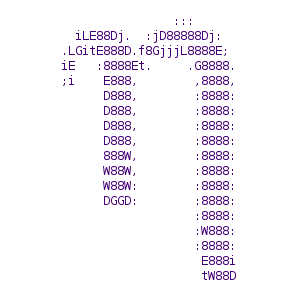
\includegraphics[width=2cm,height=2cm,scale=0.4]{nanologo.png}
	\text{(b) Nano}
	
\includegraphics[width=2cm,height=2cm,scale=0.4]{vimlogo.png}
	\text{(b) Vim}
	\caption{Terminal based text editor}
\end{figure}
\section{Equations}
In algebra, a quadratic equation is any equation having the form $ax^2+bx+c = 0$ where x represents an unknown, and a, b, and c represent known numbers, with $a \neq 0$. It can easily be seen, by polynomial expansion, that the following equation is equivalent to the quadratic equation:
$$\left({x+\frac{b}{2a}}^2\right)=\frac{b^2-4ac}{4a^2}$$
\pagebreak
\newpage
Taking the square root of both sides, and isolating x, gives:
\begin{equation}
x=\frac{-b+\sqrt{b^2-4ac}}{2a}
\end{equation}
\subsection*{Some Equations:}
$$f_1(t)=\int_{3}^5 \sin (x)dx$$
$$F(x)=A_0+ \sum_{n=1}^N\left[A_n\cos\left(\frac{2\pi nx}{P}\right)+B_n\sin\left(\frac{2\pi nx}{P}\right)\right]$$
$$\lim_{x \to a} \frac{f(x)-f(a)}{x-a}$$
$$\binom{a}{b+c} \binom{\frac{n^2-1}{2}}{n+1}$$
$$h \leq \sqrt{\frac{(s-a)(s-b)(s-c)}{s}}$$
$$6CO_2+6H_20\xrightarrow{} C_6H_{12}O_6+6O_2$$
$$\begin{bmatrix}
    a_{1}  & a_{2} & a_{3}  \\
    b_{1}  & b_{2} & b_{3} \\
    c_{1} & c_{2} & c_{3}
\end{bmatrix}$$
\section{Bibliography}
The recent success of neural networks has boosted research on pattern recognition and data mining. Many machine learning tasks such as object detection in “You Only Look Once” \cite{blah1}, machine translation \cite{blah2}, and speech recognition \cite{blah3}, which once heavily relied on handcrafted feature engineering to extract informative feature sets, has recently been revolutionized by various end-to-end deep learning paradigms, i.e., convolutional neural networks (CNNs) \cite{blah5}, long shortterm memory (LSTM) \cite{blah4}, and autoencoders.
\pagebreak
\printbibliography
\end{document}